\documentclass[12pt]{article}
\usepackage[utf8]{inputenc}
\usepackage{upquote}
\usepackage[margin=20mm]{geometry} 
\usepackage{amsmath,amsthm,amssymb}
\usepackage{graphicx}
\usepackage{listings}
\newenvironment{statement}[2][Statement]{\begin{trivlist}
\item[\hskip \labelsep {\bfseries #1}\hskip \labelsep {\bfseries #2.}]}{\end{trivlist}}
\usepackage{xcolor}

\usepackage{subfigure}


% Listings package for code rendering (No external dependencies)
\usepackage{listings}  
\usepackage{xcolor}   % Color support
\usepackage{tcolorbox} % Box for better appearance

% Define custom colors for code highlighting
\definecolor{codegreen}{rgb}{0,0.6,0}
\definecolor{codegray}{rgb}{0.5,0.5,0.5}
\definecolor{codepurple}{rgb}{0.58,0,0.82}
\definecolor{backcolour}{rgb}{0.95,0.95,0.92}


\lstset{frame=tb,
    language=Python,
    backgroundcolor=\color{backcolour},   
    commentstyle=\color{codegreen},
    keywordstyle=\color{magenta},
    numberstyle=\tiny\color{codegray},
    stringstyle=\color{codepurple},
    basicstyle=\ttfamily\footnotesize,
    breakatwhitespace=false,         
    breaklines=true,                 
    keepspaces=true,                 
    numbers=left,       
    numbersep=5pt,                  
    showspaces=false,                
    showstringspaces=false,
    showtabs=false,                  
    tabsize=2,
}





\title{Assignment 7}


\author{Author \\
 Wanjing Hu / fng685@alumni.ku.dk  \\
 Shuangcheng Jia / bkg713@alumni.ku.dk/   \\
 Zhigao Yan / sxd343@alumni.ku.dk  \\
} 

\begin{document}
\maketitle

\section{Segmentation}
%shuangcheng

\section{Image Transform}
%shuangcheng

\section{The Hough Transform}
%zhigao
\subsection{}
\begin{lstlisting}
    def hough_transform(edge_image, theta_step=1, rho_step=1, threshold=100):
    # Chose range and discretization of \rho and \theta.
    rows, cols = edge_image.shape
    diagonal = int(np.ceil(np.sqrt(rows**2 + cols**2)))  # Edge image diagonal length
    thetas = np.deg2rad(np.arange(0, 180, theta_step))   # theta : 0-180 degree
    rhos = np.arange(-diagonal, diagonal, rho_step)      # rho : [-d, d]
    
    # Create accumulator 2D array (Hough Space)
    accumulator = np.zeros((len(rhos), len(thetas)), dtype=np.uint64)
    
    # Iterate over all edge pixels
    edge_points = np.argwhere(edge_image)  # Get all the edge coordinates [y, x]
    
    for (y, x) in edge_points:            # Iterate over each edge point
        for theta_idx, theta in enumerate(thetas):  
            # Calculate the corresponding value of \rho
            rho = x * np.cos(theta) + y * np.sin(theta)
            
            # Ensure that the accumulator array index cannot be negative
            rho_idx = int(round((rho + diagonal) / rho_step))
            
            # Updating the accumulator (to ensure that it does not go out of bounds)
            if 0 <= rho_idx < len(rhos):
                accumulator[rho_idx, theta_idx] += 1
    
    # Lines correspond to accumulator values larger than a certain threshold.
    lines = []
    for rho_idx in range(accumulator.shape[0]):
        for theta_idx in range(accumulator.shape[1]):
            if accumulator[rho_idx, theta_idx] >= threshold:
                lines.append( (rhos[rho_idx], thetas[theta_idx]) )
    
    return lines, accumulator
\end{lstlisting}
The code is written strictly following the steps on slide.
Firstly input the edge image, the step size and the threshold value. Determine the range of $ \theta $ and $ \rho $ according to the steps in slide.
Then the first iteration is performed and the corresponding $ \rho $ is computed. the second iteration gets the lines that are greater than the threshold.


Computational complexity (two iterations): 
\[ O(E \times T) + O(R \times T) \]
E: indicates the number of edge pixels.
T: The number of $ \theta $
R: The number of all calculated $ \rho $ in the accumulator

\subsection{}
\begin{figure}[ht]
    \centering
    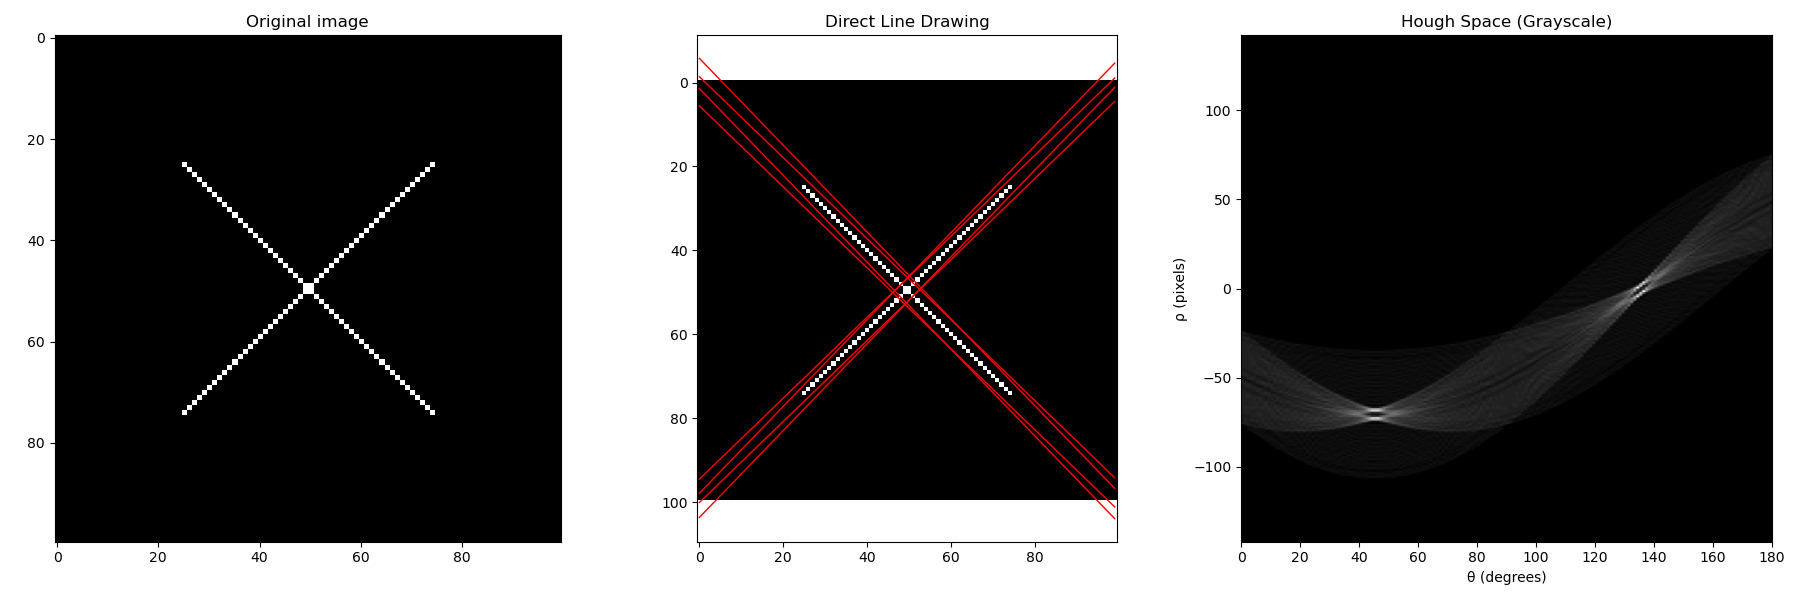
\includegraphics[width=0.7\textwidth]{pics/A7_3.2_1.png} 
    \caption{Hough Transform by my implementation}
    \label{fig: Figure 1}
\end{figure}
\begin{figure}[ht]
    \centering
    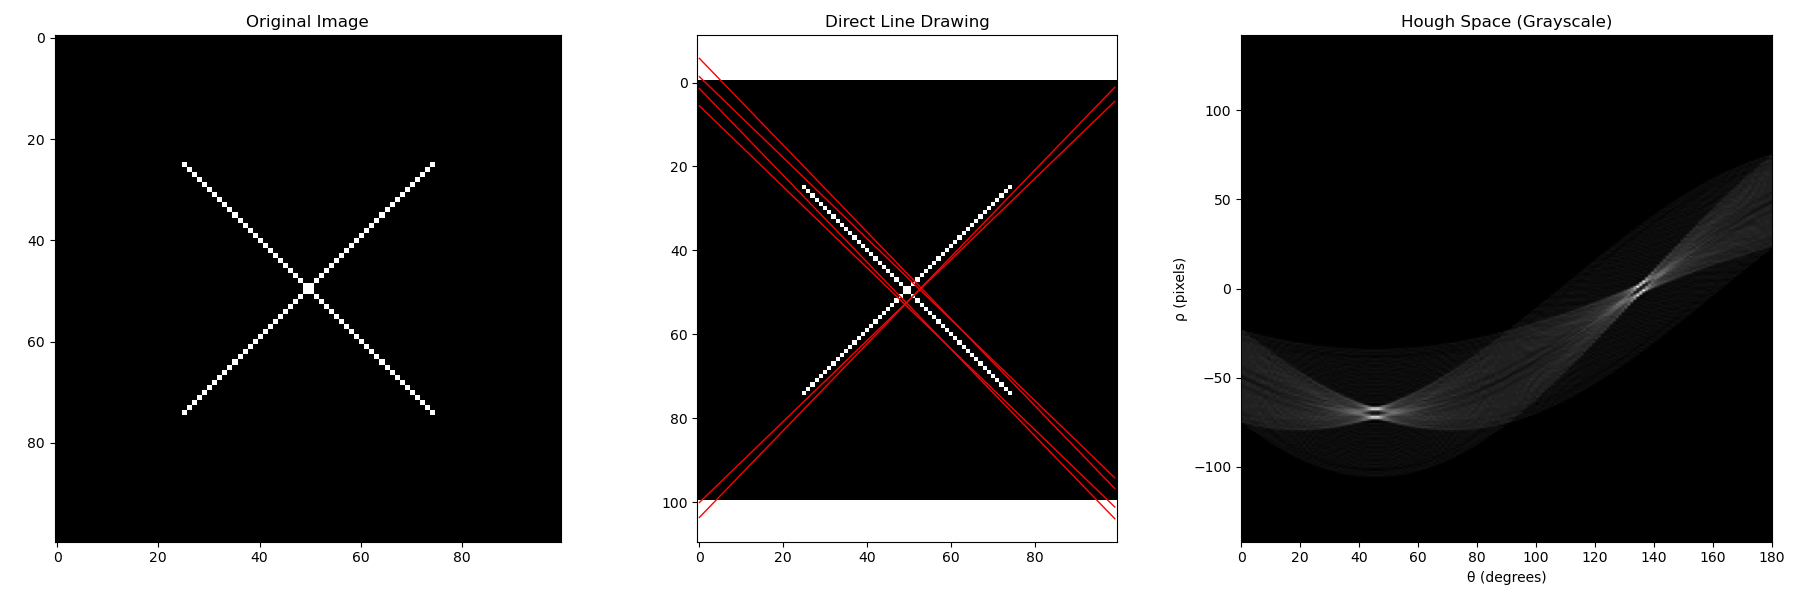
\includegraphics[width=0.7\textwidth]{pics/A7_3.2_2.png} 
    \caption{Hough Transform by skimage}
    \label{fig: Figure 2}
\end{figure}
First of all, my implementation and skimga's implementation output the same Hough transform.
But as can be seen in Figures \ref{fig: Figure 1} and \ref{fig: Figure 2}, my method outputs more lines for the same threshold.
I think there may be a difference in the method of calculation, skimage's method may filter adjacent peaks resulting in fewer lines.
\subsection{}
\begin{figure}[ht]
    \centering
    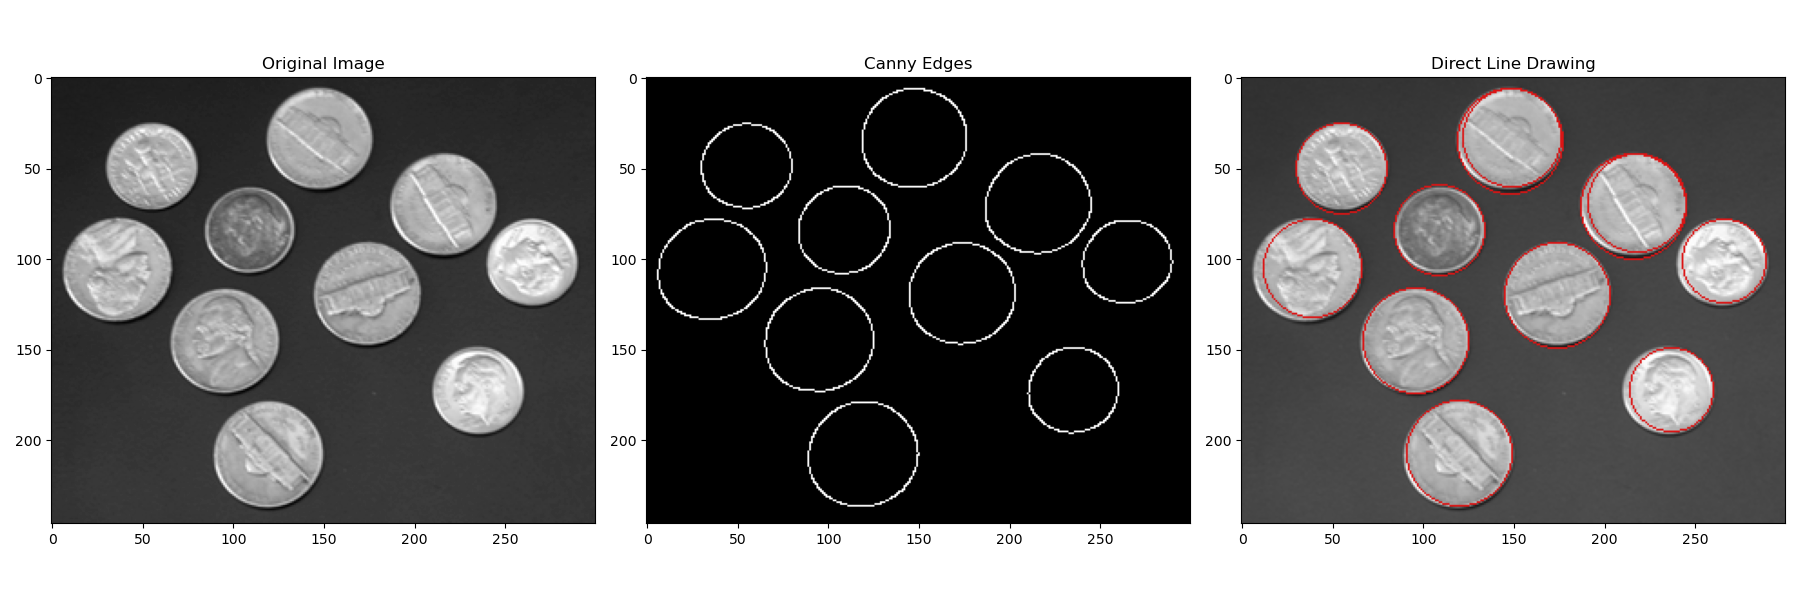
\includegraphics[width=0.8\textwidth]{pics/A7_3.3.png} 
    \caption{Hough circle by skimage}
    \label{fig: Figure 3}
\end{figure}
First use the Canny method to get the edge graph.
Then set a radius range, based on the size of the coin in the picture. 
The next step is to call the hough-circle method to get the accumulator, and finally call hough-circle-peaks to get the most obvious circle and draw it.
\subsection{}


\section{Morphology}
%wanjing
\subsection{} % 4.1

\subsubsection{Applying Opening and Closing} % 4.1.1 

Figure~\ref{fig:full_images} \textit{Original} shows the original image, as well as the results of the opening and closing operations in \textit{Opened} and \textit{Closed} (Here we choose disk=1). A zoomed-in region is presented in Figure~\ref{fig:full_images} \textit{Zoom}, \textit{Opened Zoom} and \textit{Closed Zoom} to highlight local changes.

\textbf{Changes: } As shown in the space around largest white spot, the \textit{Opened} removes small white specks and breaks thin connections, and the \textit{Closed} fills small black holes and merges nearby regions.

\begin{figure}[ht]
    \centering
        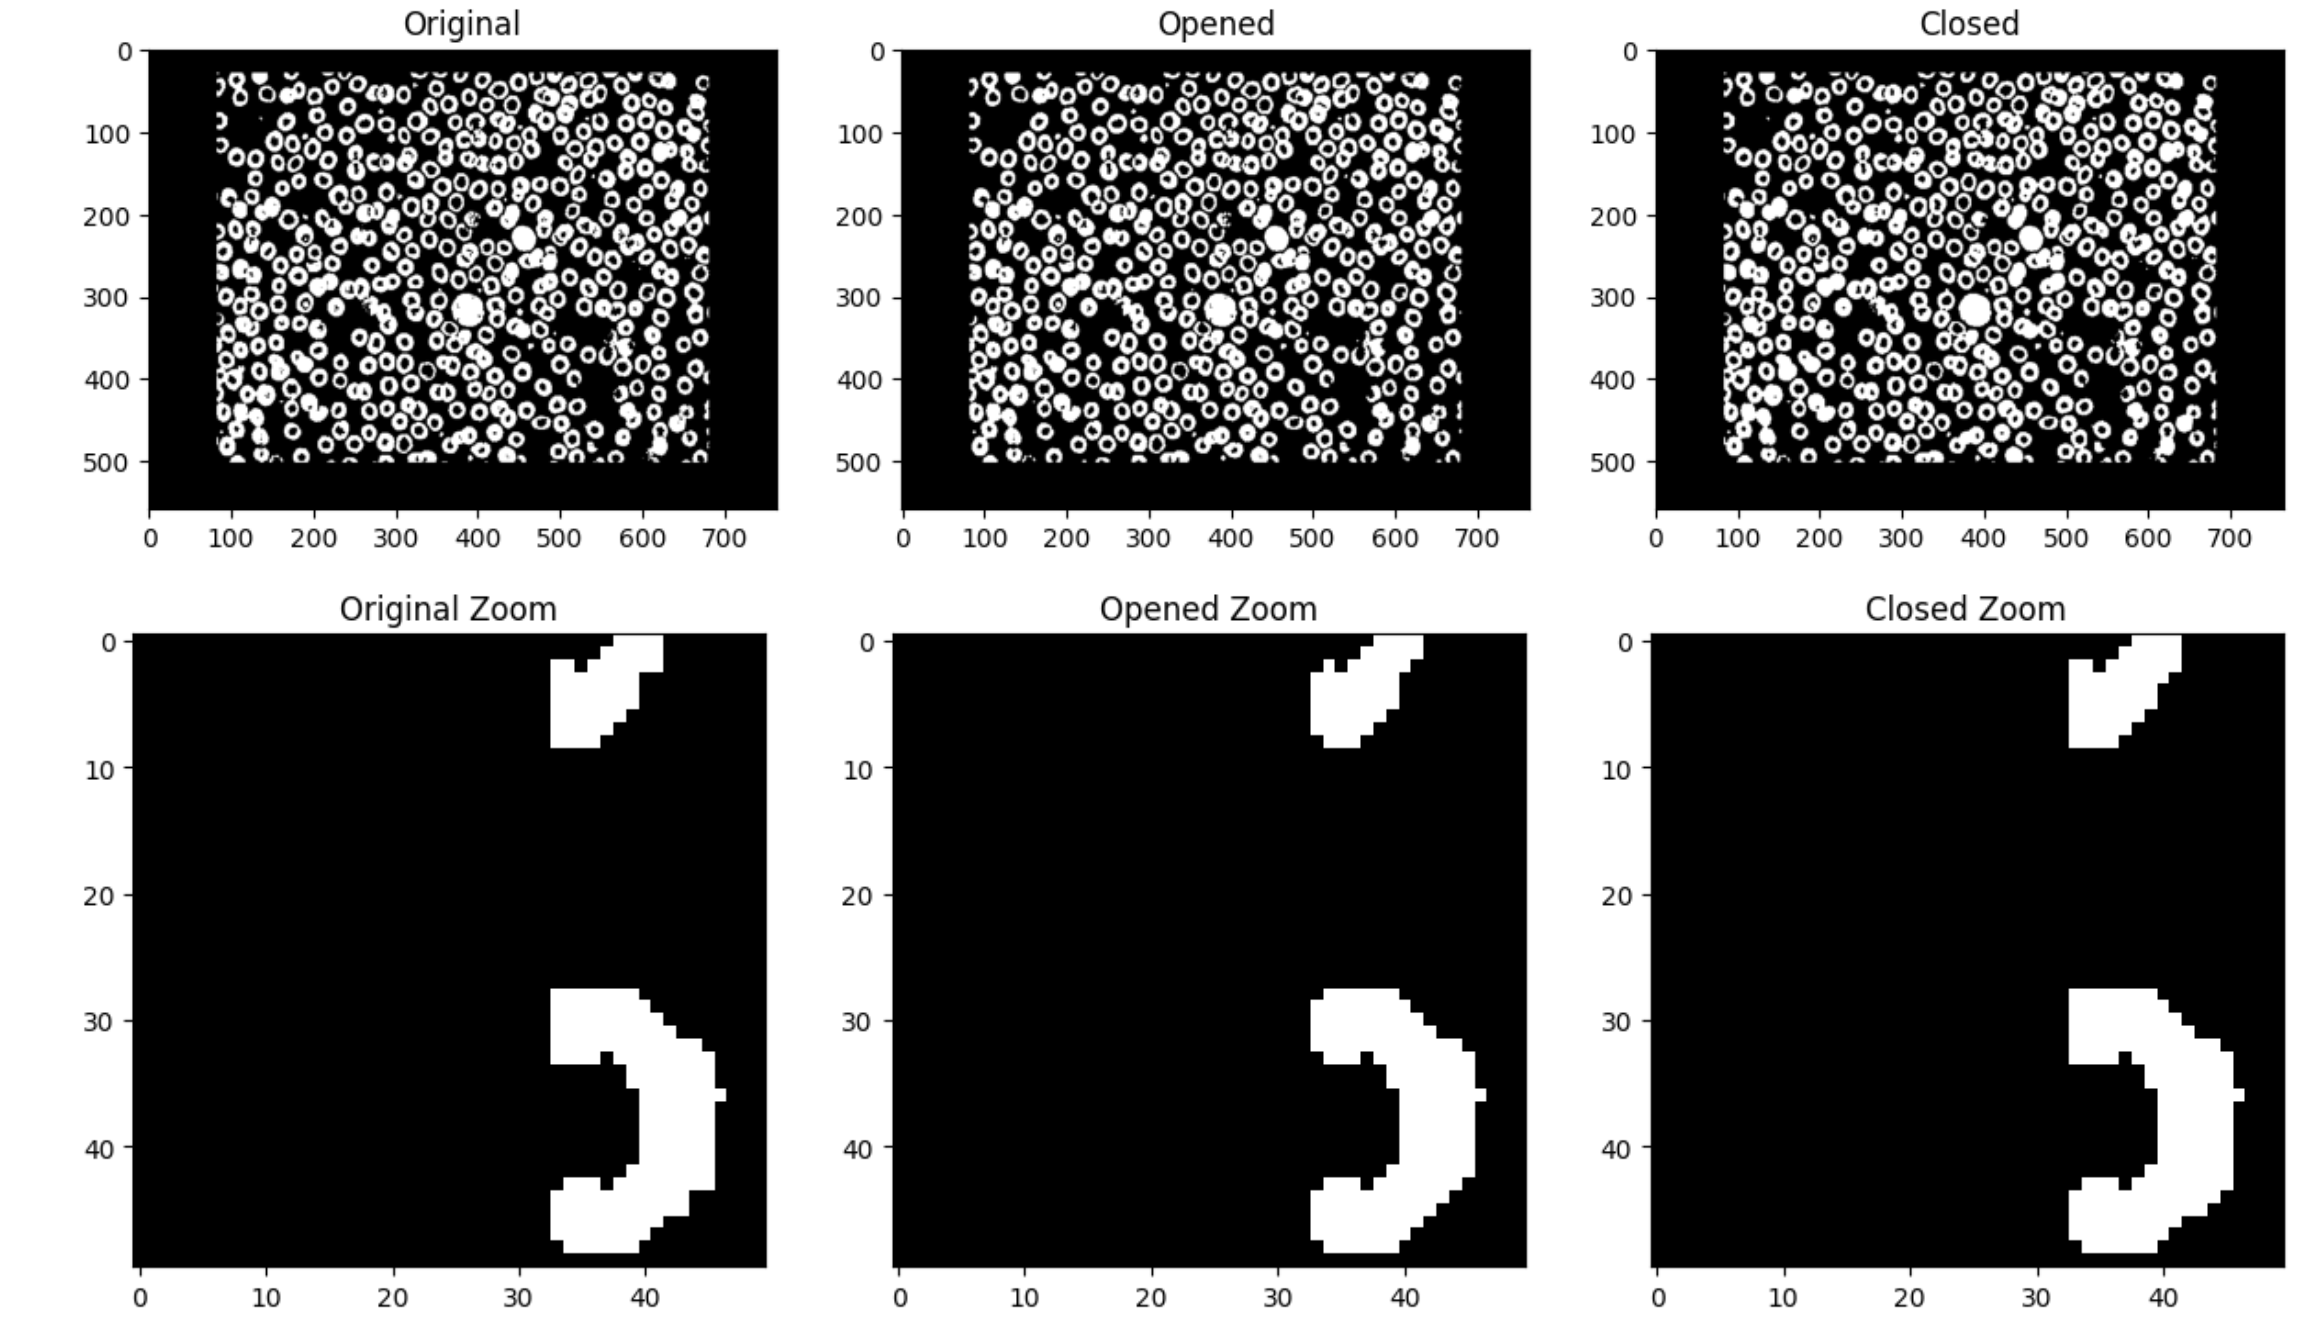
\includegraphics[width=0.9\textwidth]{pics/a7-4.1.1}
    \caption{Original and Morphologically Processed Images}
    \label{fig:full_images}
\end{figure}


\subsubsection{Differences and Challenges} % 4.1.2 
\textbf{A. } As noted in the course material \textit{Mathematical morphology - properties of dilation and erosion} page 17, opening and closing are dual operations; opening erodes then dilates (removing small bright objects), while closing dilates then erodes (filling small dark holes). In this case, opening reduces small cell fragments and isolates larger structures, whereas closing connects adjacent components and fills gaps.

\textbf{B. } When separating individual cells with those methods, some cells remain connected after closing, making separation difficult, and then opening may remove small structures that are actually part of valid cells. Also, these operations are not sufficient to segment overlapping or touching cells completely.

\subsubsection{Connected Components Analysis} % 4.1.3 

Figure \ref{fig:connected_components} shows the labeled images. For the different connected components, Opened image yields more labels (separated cells) with number=369, and the Closed image has fewer labels (merged cells), indicating over-merging, with number = 343.


\begin{lstlisting}
from skimage.measure import label

# Label connected components
labels_open = label(opened, connectivity=2)
labels_close = label(closed, connectivity=2)

print(f"Opened labels: {labels_open.max()}") # num_opened
print(f"Closed labels: {labels_close.max()}") # num_closed

# Visualize labels
plt.figure(figsize=(10,5))
plt.subplot(121).imshow(labels_open, cmap='nipy_spectral')
plt.title(f'Connected Components (Opened) - {labels_open.max()} labels')
plt.subplot(122).imshow(labels_close, cmap='nipy_spectral')
plt.title(f'Connected Components (Closed) - {labels_close.max()} labels')
plt.show()
\end{lstlisting}


\begin{figure}[ht]
    \centering
        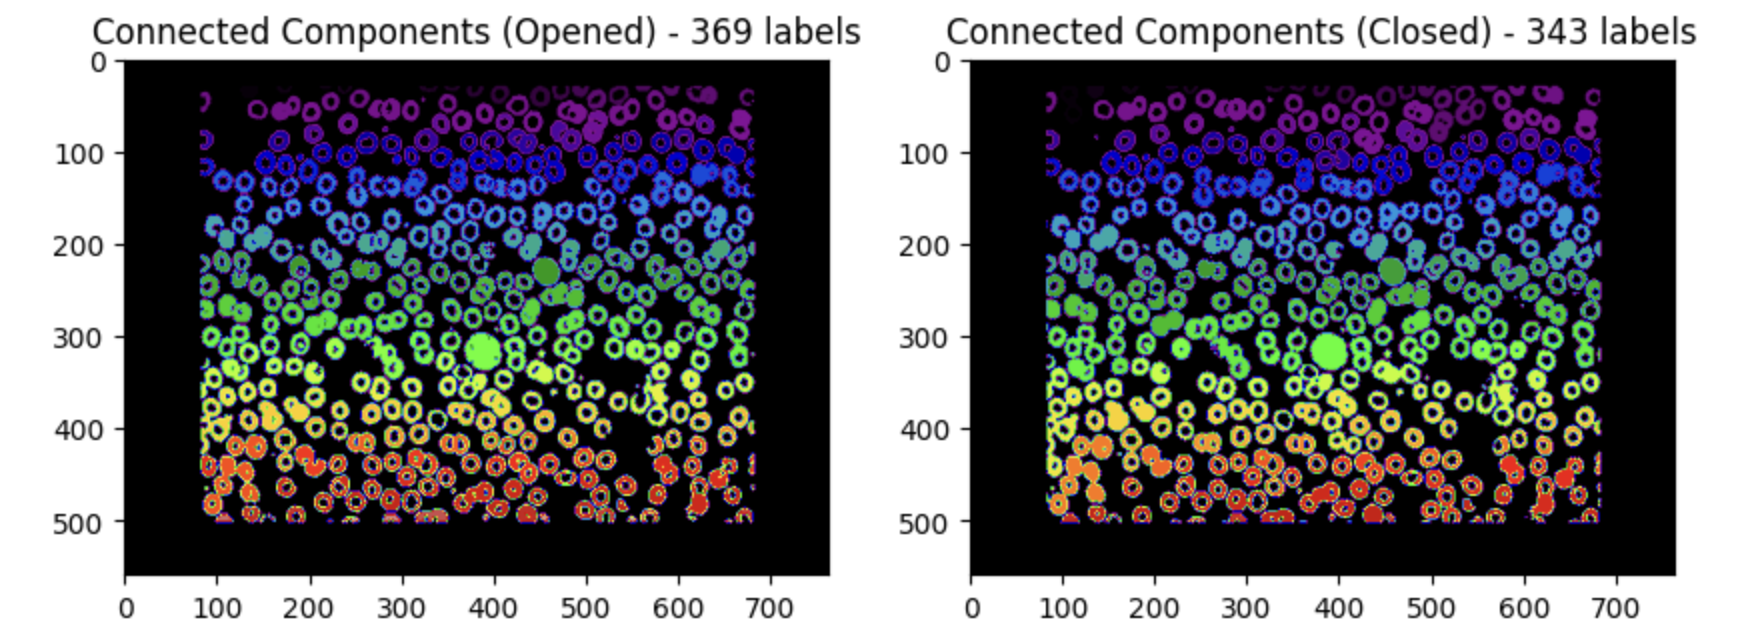
\includegraphics[width=\textwidth]{pics/a7-4.1.3}
    \caption{Connected Component Labeling Results}
    \label{fig:connected_components}
\end{figure}

\textbf{Reflection: }We find the opening operation tends to break apart connected cells, increasing the number of detected components. The closing operation joins adjacent cells, reducing the total number of detected components. Also, neither operation is fully effective at isolating individual cells, and additional techniques such as watershed segmentation may be required.

\subsection{} % 4.2

Final total amount 45 kr. What we did: First we convert he input image to a binary format by setting pixels above a certain intensity threshold to \texttt{True}. 
Then we apply Morphological Closing. The small gaps in the binary image are filled using a disk-shaped structuring element of radius 5.

Then we did Connected Component Analysis. we use the \texttt{measure.label} function and it identifies individual objects (coins) in the image using 8-connectivity.

Then we compute the Region Properties with function \texttt{measure.regionprops\_table}. It computes the area of each labeled region.

Finally the coins are assigned a denomination based on their area, and we sum up the assigned values as the total amount. Our rules of the mapping the areas to values is as follows:
    \begin{itemize}
        \item If area $> 1000$, assign 20 kr.
        \item If area $> 500$, assign 10 kr.
        \item Otherwise, assign 5 kr.
    \end{itemize}

\subsection{} % 4.3

After both trying out opening and closing, we choose the \textit{Closing (Dilation + Erosion)} to fill thin black lines (0s in the binary mask) while preserving the shape of larger structures (map outline and blue dot). The disk-shaped structuring element ensures isotropic processing to handle lines in any direction.

After trying different parameters(disk radius=1,2,3,4,5), we choose the disk of radius 2, and it is large enough to cover the thickness of the lines but small enough to avoid distorting critical features.

\begin{lstlisting}
# Define different structuring element sizes
disk_sizes = [1, 2, 3, 4, 5]

fig, axes = plt.subplots(len(disk_sizes), 3, figsize=(15, 10))

for i, size in enumerate(disk_sizes):
    selem = morphology.disk(size)

    # Perform opening and closing
    opened = morphology.opening(binary_nat, selem)
    closed = morphology.closing(binary_nat, selem)

    # Plot original, opened, and closed images
    axes[i, 0].imshow(binary_nat, cmap='gray')
    axes[i, 0].set_title(f'Original (Disk={size})')

    axes[i, 1].imshow(opened, cmap='gray')
    axes[i, 1].set_title(f'Opened (Disk={size})')

    axes[i, 2].imshow(closed, cmap='gray')
    axes[i, 2].set_title(f'Closed (Disk={size})')

plt.tight_layout()
plt.show()
\end{lstlisting}

For the result visualization, we overlay the original binary image and cleaned result and high light the difference, as shown in Figure~\ref{fig:viz}.

\begin{figure}[ht]
    \centering
        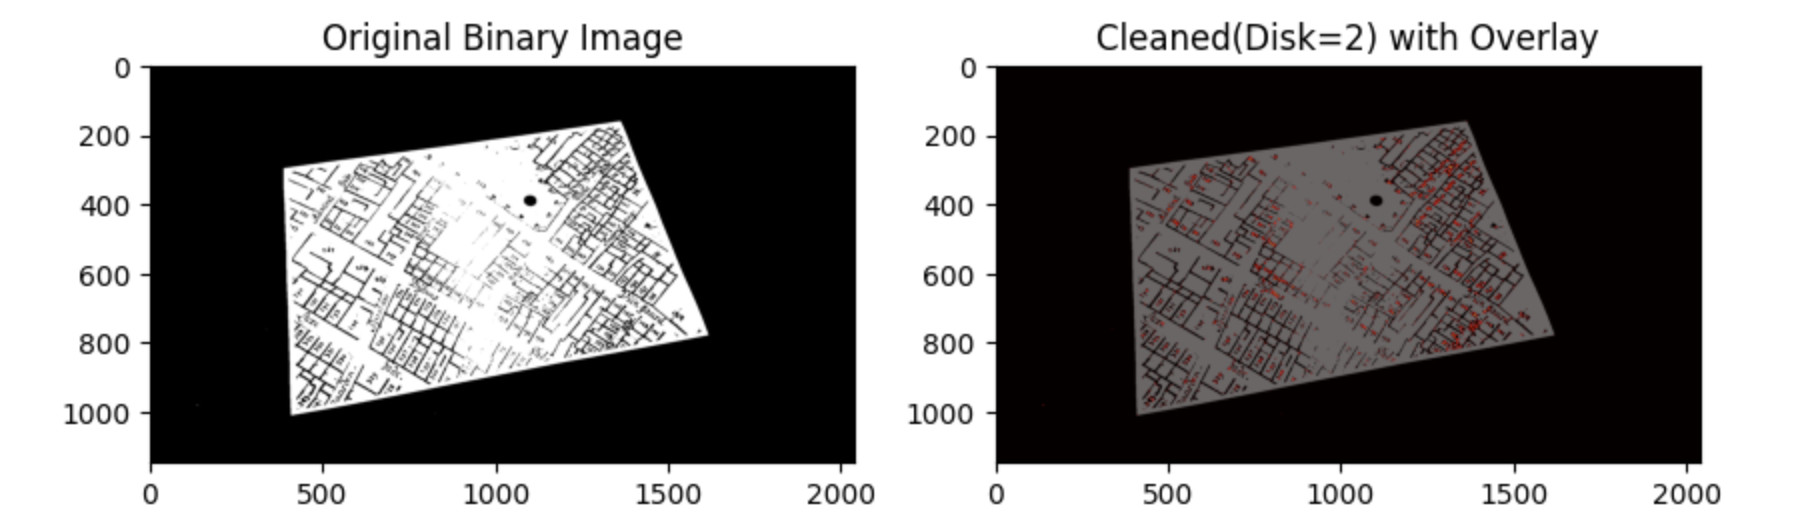
\includegraphics[width=\textwidth]{pics/a7-4.3}
    \caption{Visualization of the cleaned binary segmentation mask}
    \label{fig:viz}
\end{figure}


\end{document}
